\begin{example}[While with Two Paths]
  \label{ex:twoPathsWhile}
  %
  { \small
  \begin{figure}
  \centering
  \begin{subfigure}{.4\textwidth}
    \begin{centering}
    {\small
    $
    \begin{array}{l}
      \kw{twoPathsWhile}(n, m) \triangleq \\
    \clabel{ \assign{i}{n} }^{0} ; \\
    \clabel{ \assign{j}{0} }^{1} ; \\
        \ewhile ~ \clabel{i > 0}^{2} ~ \edo ~ \\
        \qquad \Big(
          \eif(\clabel{j < m}^{3}, \\
          \qquad \qquad \clabel{\assign{j}{j + 1}}^{4}; 
          \clabel{\assign{i}{i - 1}}^{5},\\
          \qquad \qquad \clabel{\assign{j}{0}}^{6});
          \Big)
        \end{array}
        $
    }
    \caption{}
    \end{centering}
    \end{subfigure}
  \begin{subfigure}{.5\textwidth}
    \begin{centering}
  %   \todo{abstract-cfg for two round}
  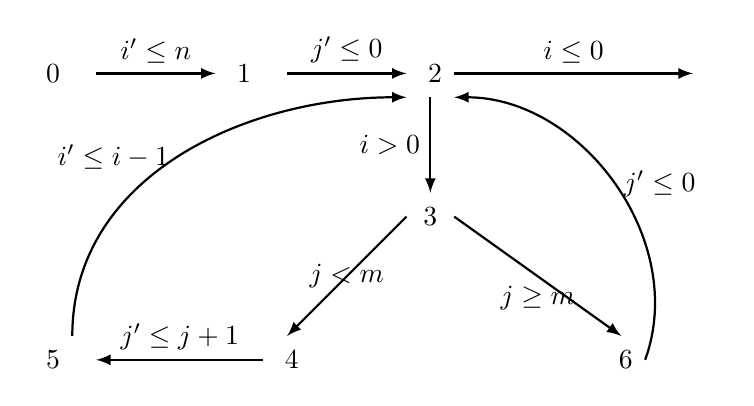
\begin{tikzpicture}[scale=\textwidth/20cm,samples=200]
  \draw[] (-8, 10) circle (0pt) node{{ $0$}};
  \draw[] (-4, 10) circle (0pt) node{{ $1$}};
  \draw[] (0, 10) circle (0pt) node{{ $2$}};
  \draw[] (0, 7) circle (0pt) node{{$3$}};
  \draw[] (-3, 4) circle (0pt) node{{ $4$}};
  \draw[] (-8, 4) circle (0pt) node{{ $5$}};
  \draw[] (4, 4) circle (0pt) node{{ $6$}};
  % Counter Variables
  \draw[] (6, 10) circle (0pt) node {\textbf{$\lex$}};
  % \draw[] (6, 4) circle (0pt) node {{ $ex$}};
  %
  % Control Flow Edges:
  \draw[ thick, -latex] (-7, 10)  -- node [above] {$i' \leq n$}(-4.5, 10);
  \draw[ thick, -latex] (-3, 10)  -- node [above] {$j' \leq 0$}(-0.5, 10);
  \draw[ thick, -latex] (0, 9.5)  -- node [left] {$i > 0$} (0, 7.5) ;
  \draw[ thick, -latex] (0.5, 7)  -- node [below] {$ j \geq m $}  (4, 4.5);
  \draw[ thick, -latex] (-7.5, 4.5)  to  [out=90,in=180]  node [left] {$i' \leq i - 1$ }(-0.5, 9.5);
  \draw[ thick, -latex] (4.5, 4)  to  [out=70,in=0]   node [right] {$j' \leq 0 $}(0.5, 9.5);
  \draw[ thick, -latex]  (-0.5, 7) -- node  {$j < m$}  (-3, 4.5) ;
  \draw[ thick, -latex]  (-3.5, 4) -- node [above] {$j' \leq j + 1$}  (-7, 4) ;
  \draw[ thick, -latex] (0.5, 10)  -- node [above] {$i \leq 0$}  (5.5, 10);
  % \draw[ thick, -latex] (6, 6.5)  -- node [right] {$\top$} (6, 4.5) ;
  \end{tikzpicture}
  \caption{}
    \end{centering}
    \end{subfigure}
  \caption{
  (a) The Two Paths While Loop Example
    (b) The Abstract Execution Control Flow Graph}
      \label{fig:twoPathsWhile}
  \end{figure}
  }
\end{example}

\begin{enumerate}
  \item  \textbf{The Abstract Control Flow Graph}: Figure~\ref{fig:twoPathsWhile}(b).

  \item \textbf{Program Refinement}:
  \\
  {Simple Transition Paths:\footnote{For concise, the edges sequence and the constraint on each edge in
  each transition path are omitted.}}
  \\
$
\begin{array}{llll}
  \tpath_0 = (0 \to 1 \to 2)
  &
  \tpath_2 = (2 \to 3 \to 6 \to 2)
  &
  \tpath_1 = (2 \to 3 \to 4 \to 5 \to 2)
  &
  \tpath_3 = (2 \to \lex)
  \end{array}
$\footnote{We use the notation $(l_0 \to \ldots \to l_n)$ to denote a vertices sequence $(l_0, \ldots, l_n)$.}
\\
{Refined Program:\footnote{The program $c$ and its refined program $\rprog$ is used as the inputs (/ arguments) of the computations in the following steps.
For concise, it is omitted since all the arguments in the following computations are referring to the same program.}}
\\
$
  \tpath_0 ; 
  \rpchoose{2: \rprepeat_2(\rprepeat_1(\tpath_1); \tpath_2) , 
  2: \rprepeat_1(\tpath_1) }; \tpath_3
$
%
\item {Path Local Reachability-bound}:
\\
$\outinB(\rpchoose{2: \rprepeat_2(\rprepeat_1(\tpath_1); \tpath_2) , 
2: \rprepeat_1(\tpath_1) } , \tpath_1) = \max\{m, m \times \lfloor\frac{n}{m}\rfloor\}$ 
\\
$\outinB(\rpchoose{2: \rprepeat_2(\rprepeat_1(\tpath_1); \tpath_2) , 
2: \rprepeat_1(\tpath_1) }, \tpath_2) = \lfloor\frac{n}{m}\rfloor$ 
%
\\
Loop Bounds:
\\
     $ BD(\tpath_0) = 1$
      \quad
      $BD(\rprepeat_1(\tpath_1)) = m $
      \quad
      $BD(\rprepeat_2(\rprepeat_1(\tpath_1); \tpath_2)) = \lfloor\frac{n}{m}\rfloor$
%
\item Path Global Reachability-bound:
\\
$\inoutB(\rprog, \tpath_1) = \max\{m, m \times \lfloor\frac{n}{m}\rfloor\}$ \quad
$\inoutB(\rprog, \tpath_2) = \lfloor\frac{n}{m}\rfloor$ \quad
$\inoutB(\rprog, \tpath_0) = \inoutB(\rprog, \tpath_3) = 1$ 
%
\item Loop Reachability-bound:
No nested loop.%
\item The Reachability-bound:
\\
$\psRB(0) = \psRB(1) = \psRB(\lex) = 1$ \qquad
$\psRB(4) = \psRB(5) = \max\{m, m \times \lfloor\frac{n}{m}\rfloor\}$ 
\\
$\psRB(3) = \psRB(2) = \max\{m, m \times \lfloor\frac{n}{m}\rfloor\} + \lfloor\frac{n}{m}\rfloor + 1 $
\quad $\psRB(6) = \lfloor\frac{n}{m}\rfloor$  
\end{enumerate}